\documentclass[UTF8,a4paper,11pt]{ctexart}
\usepackage[a4paper,margin=2.0cm,headheight=16pt]{geometry}
\usepackage{graphicx,booktabs,tabularx,longtable,array,amsmath,amssymb,multirow}
\usepackage[table]{xcolor}
\usepackage{hyperref,fancyhdr,titlesec,enumitem,float,caption,subcaption,listings,microtype,setspace,seqsplit}
\usepackage{tikz}
\usetikzlibrary{arrows.meta,positioning,fit,backgrounds}
\setCJKmainfont{Noto Serif CJK SC}
\setCJKsansfont{Noto Sans CJK SC}
\setmainfont{TeX Gyre Pagella}
\setsansfont{TeX Gyre Heros}
\setmonofont{DejaVu Sans Mono}

\definecolor{RadarBlue}{HTML}{3777FF}
\definecolor{RadarCyan}{HTML}{20C7AA}
\definecolor{RadarNavy}{HTML}{102039}
\definecolor{RadarOrange}{HTML}{FF9D42}
\definecolor{RadarRed}{HTML}{E65362}
\definecolor{RadarGreen}{HTML}{159F72}
\definecolor{LightBlue}{HTML}{EEF4FF}
\definecolor{LightGreen}{HTML}{EAF8F2}
\definecolor{LightOrange}{HTML}{FFF3E8}
\definecolor{LightGray}{HTML}{F5F7FA}

\hypersetup{
  colorlinks=true,linkcolor=RadarBlue,urlcolor=RadarBlue,citecolor=RadarCyan,
  pdftitle={RadarMind-DriveLM 六视角 Graph-VLM 技术演进报告},
  pdfauthor={RadarMind Project / 张宗元}
}
\graphicspath{{assets/}}
\captionsetup{font=small,labelfont=bf}
\setlength{\parindent}{2em}
\setlength{\parskip}{0.32em}
\setlength{\emergencystretch}{2em}
\setlist{nosep,leftmargin=2em}
\renewcommand{\arraystretch}{1.18}
\newcolumntype{Y}{>{\raggedright\arraybackslash}X}
\newcolumntype{C}{>{\centering\arraybackslash}X}
\newcommand{\code}[1]{\texttt{\small #1}}
\newcommand{\metric}[1]{\textbf{\color{RadarBlue}#1}}
\newcommand{\winner}{\textbf{\color{RadarGreen}晋级}}
\newcommand{\reject}{\textbf{\color{RadarRed}未晋级}}
\titleformat{\section}{\Large\bfseries\sffamily\color{RadarNavy}}{\thesection}{0.65em}{}
\titleformat{\subsection}{\large\bfseries\sffamily\color{RadarBlue}}{\thesubsection}{0.55em}{}
\titleformat{\subsubsection}{\normalsize\bfseries\sffamily\color{RadarNavy}}{\thesubsubsection}{0.5em}{}
\titlespacing*{\section}{0pt}{1.3em}{0.6em}
\titlespacing*{\subsection}{0pt}{1.0em}{0.4em}
\pagestyle{fancy}
\fancyhf{}
\fancyhead[L]{\small\sffamily RadarMind $\times$ DriveLM}
\fancyhead[R]{\small\sffamily Graph-VLM 技术演进报告 v2.0}
\fancyfoot[C]{\thepage}
\renewcommand{\headrulewidth}{0.4pt}
\lstdefinestyle{code}{
  basicstyle=\ttfamily\footnotesize,backgroundcolor=\color{LightGray},
  frame=single,rulecolor=\color{LightGray},breaklines=true,
  columns=fullflexible,keepspaces=true,showstringspaces=false,
  xleftmargin=0.5em,xrightmargin=0.5em
}
\lstset{style=code}

\begin{document}
\begin{titlepage}
  \pagecolor{RadarNavy}\color{white}
  \vspace*{1.0cm}
  {\sffamily\Large RadarMind Project\par}
  \vspace{0.35cm}
  {\noindent\color{RadarCyan}\rule{\textwidth}{2pt}\par}
  \vspace{1.25cm}
  {\sffamily\bfseries\fontsize{28}{36}\selectfont
  RadarMind-DriveLM\\[0.20em]六视角 Graph-VLM 技术演进报告\par}
  \vspace{0.75cm}
  {\sffamily\fontsize{17}{25}\selectfont
  从零样本基模、垂域 SFT、DPO、Mixture of LoRA、\\
  Trajectory RL 到 Graph 专家路由的完整可复现链路\par}
  \vfill
  \begin{tabular}{ll}
    报告版本：& v2.0（覆盖项目 v0.31--v0.44）\\
    项目作者：& 张宗元\\
    更新日期：& 2026-08-18\\
    发布仓库：& \texttt{radarmind-drivelm}\\
    当前基线：& v0.43 Graph anchor + MoL downstream\\
  \end{tabular}
  \vspace{1.0cm}

  {\small 本报告只使用可由本地 JSON、日志、checkpoint 与代码复核的结果。\\
  3,355 条指标来自 scene-isolated local dev；语义裁判为 DeepSeek-V4-Flash 代理，\\
  不是官方隐藏服务器的 ChatGPT 分数。\par}
\end{titlepage}
\nopagecolor\color{black}

\begin{abstract}
本报告总结 RadarMind-DriveLM 从最初数据复现到完整 Graph-VLM Agent 的技术演进。项目以 DriveLM-nuScenes v1.1 为数据基础，将单帧六路同步相机图像组织为 26,095 条训练 QA 与 3,355 条场景隔离开发集 QA，覆盖 Perception、Prediction、Planning、Behavior 四类任务。模型主线由 Qwen2.5-VL-7B-Instruct 出发，依次完成纯交叉熵 LoRA SFT、任务均衡且带 CE anchor 的保守 DPO、四任务 Mixture of LoRA（MoL）、Planning trajectory GRPO/GSPO、四阶段 Graph trajectory SFT，以及受 InternVL4Drive 启发的固定专家路由。

零样本基模的本地 DriveLM-DS Final 为 0.257961；六相机垂域 CE-SFT 提升到 0.594636；保守 DPO 提升到 0.596356；四专家 MoL 提升到 0.608245。GRPO/GSPO 在 Planning 子协议上改善 trajectory reward，但接回完整系统后未超过 MoL。Graph-SFT 显著改善坐标 grounding，却因 teacher forcing 与 predicted-context 的暴露偏差未通过 same-ID 晋级门槛。最终系统把 Graph-A 只用于每帧第一个重要对象 anchor，把 MoL-700 用于其余 2,888 条下游 QA，在 3,355 条完整开发集上取得 0.612293；严格 1,848-ID 共同子集 Final 同样由 0.609563 提升到 0.610557。因此 v0.43 是当前本地全系统基线。

报告同时保留具有方法论价值的负实验：增加视觉 token、标准 DPO、grounding DPO、全系统 GRPO/GSPO、Graph+anchor 混合训练、显式六相机拓扑提示和 image-only bbox 辅助监督均未通过冻结晋级门槛。这些结果共同说明：DriveLM 的主要困难不是单一语言指标，而是 graph gating、对象召回、任务梯度冲突和上游误差传播；可靠模型选择必须结合完整 Final、predicted-context rollout 与 same-ID 公平审计。
\end{abstract}

\tableofcontents
\clearpage

\section{项目目标与最终系统}
\subsection{问题定义}
DriveLM 将自动驾驶推理表示为 Graph Visual Question Answering（Graph-VQA）。模型不仅需要描述场景，还要围绕关键对象完成四类任务：
\begin{itemize}
  \item \textbf{Perception：}识别影响驾驶决策的车辆、行人、骑行者和交通元素，并判断对象状态；
  \item \textbf{Prediction：}推断对象类别、运动趋势与自车未来位置需要关注的对象；
  \item \textbf{Planning：}生成候选动作、碰撞风险动作与安全动作；
  \item \textbf{Behavior：}从选项中判断自车速度与转向组合。
\end{itemize}
项目目标不是把每条 QA 独立做成普通图文问答，而是构建能够沿
\(
\small\text{Perception}\rightarrow\text{Prediction}\rightarrow\text{Planning}\rightarrow\text{Behavior}
\)
传播工作记忆的感知决策 Agent，并用接近官方结构的指标验证其完整系统性能。

\subsection{当前部署结构}
最终 v0.43 没有同时加载四个完整 VLM。系统共享一个 7B 基座，在推理时挂载任务适配器，并使用固定、无答案依赖的路由：每帧 \code{qa\_index=0} 的 important-object anchor 由 Graph-A 生成，其余 QA 由 MoL-700 的任务专家生成。

\begin{figure}[H]
\centering
\begin{tikzpicture}[scale=0.94,transform shape,
  node distance=8mm and 8mm,
  box/.style={draw=RadarBlue,rounded corners,fill=LightBlue,minimum height=10mm,align=center,font=\small},
  good/.style={draw=RadarGreen,rounded corners,fill=LightGreen,minimum height=10mm,align=center,font=\small},
  arrow/.style={-{Latex[length=2.2mm]},thick,color=RadarNavy}
]
\node[box] (cams) {六路同步相机\\独立图像输入};
\node[box,right=of cams] (base) {Qwen2.5-VL-7B\\共享基座};
\node[good,right=of base,yshift=10mm] (anchor) {Graph-A adapter\\467 条 frame anchor};
\node[good,right=of base,yshift=-10mm] (mol) {MoL-700\\2,888 条下游 QA};
\node[box,right=of anchor,xshift=7mm] (gate) {Graph gating\\对象坐标匹配};
\node[box,right=of mol,xshift=7mm] (tasks) {Prediction / Planning\\Behavior / tag-3};
\node[good,right=of gate,yshift=-10mm] (out) {DriveLM 输出\\3,355/3,355};
\draw[arrow] (cams)--(base);
\draw[arrow] (base)--(anchor);
\draw[arrow] (base)--(mol);
\draw[arrow] (anchor)--(gate);
\draw[arrow] (mol)--(tasks);
\draw[arrow] (gate)--(out);
\draw[arrow] (tasks)--(out);
\end{tikzpicture}
\caption{当前 v0.43 系统：共享基座、固定 anchor 专家与任务 LoRA 专家。路由规则不读取参考答案、候选文本或 dev 得分。}
\end{figure}

\noindent\colorbox{LightGreen}{\parbox{\dimexpr\textwidth-2\fboxsep\relax}{
\textbf{最终结论：}完整 3,355-QA Final 为 \metric{0.612293}；相对 MoL-700 的 0.608245 绝对提升 0.004048。严格 1,848-ID 共同子集 Final 仍提升 0.000993，因此不是 graph gating 改变题目集合造成的虚假增益。}}

\section{数据、拆分与训练输入}
\subsection{数据来源}
训练标注来自 DriveLM-nuScenes v1.1，视觉输入为同一关键帧的六路相机：
\begin{center}\small
CAM\_FRONT、CAM\_FRONT\_LEFT、CAM\_FRONT\_RIGHT；\\
CAM\_BACK、CAM\_BACK\_LEFT、CAM\_BACK\_RIGHT。
\end{center}
项目保留六图独立输入，不把六相机强制拼成单张 mosaic。这样可避免额外缩放、视角边界和单图动态切片造成的信息损失。

\begin{figure}[H]
  \centering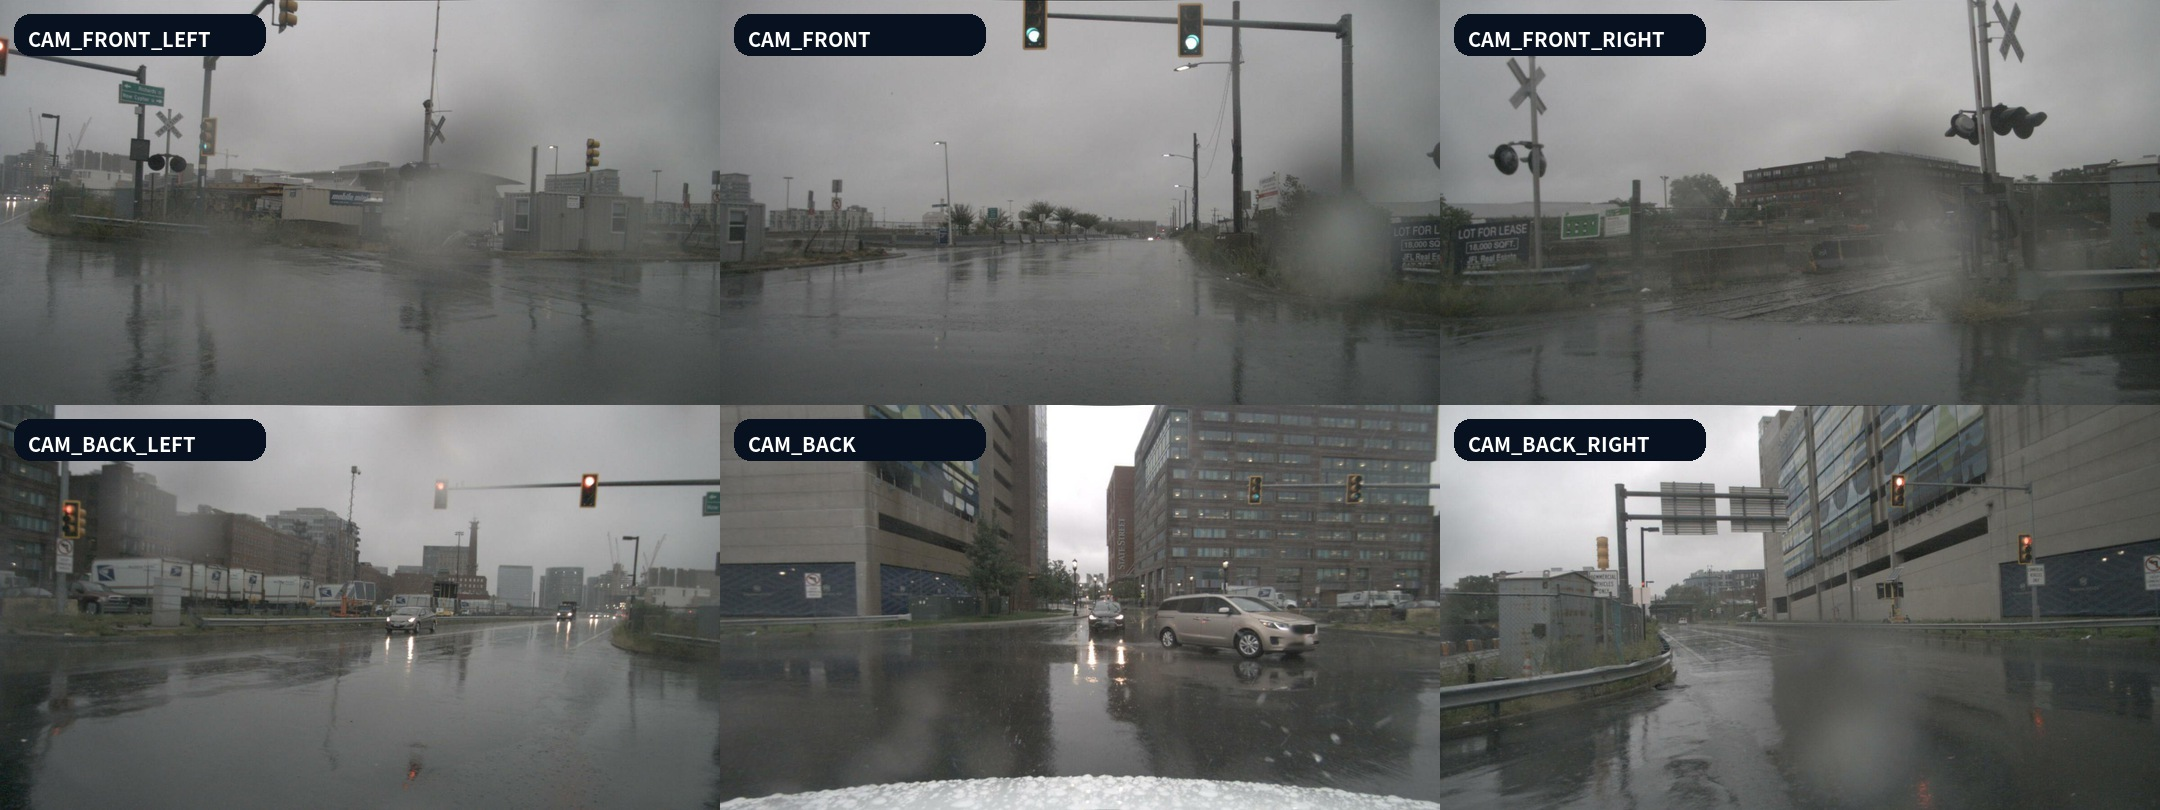
\includegraphics[width=0.94\textwidth]{six_camera_input.jpg}
  \caption{同一关键帧的六路同步图像。训练和推理中的相机顺序固定。}
\end{figure}

\subsection{场景级隔离拆分}
对 scene token 计算 SHA-256 哈希桶：
\[
b(s)=\frac{\operatorname{int}(\operatorname{SHA256}(s)_{0:8},16)}{2^{32}-1}.
\]
当 \(b(s)<0.1\) 时整个场景进入 dev，否则进入 train。同一约 20 秒场景的相邻关键帧不会跨越训练和开发集。

\begin{table}[H]
\centering
\caption{当前主线数据规模。}
\begin{tabular}{lrrrr}
\toprule
划分 & 场景数 & Frame trajectory & QA 数 & 用途\\
\midrule
Train & 619 & 3,605 & 26,095 & SFT / DPO / MoL / Graph\\
Local dev & 77 & 467 & 3,355 & 本地生成、筛选与公平审计\\
Official val & 149 & -- & 15,480 & 无答案提交集\\
\bottomrule
\end{tabular}
\end{table}

\begin{figure}[H]
  \centering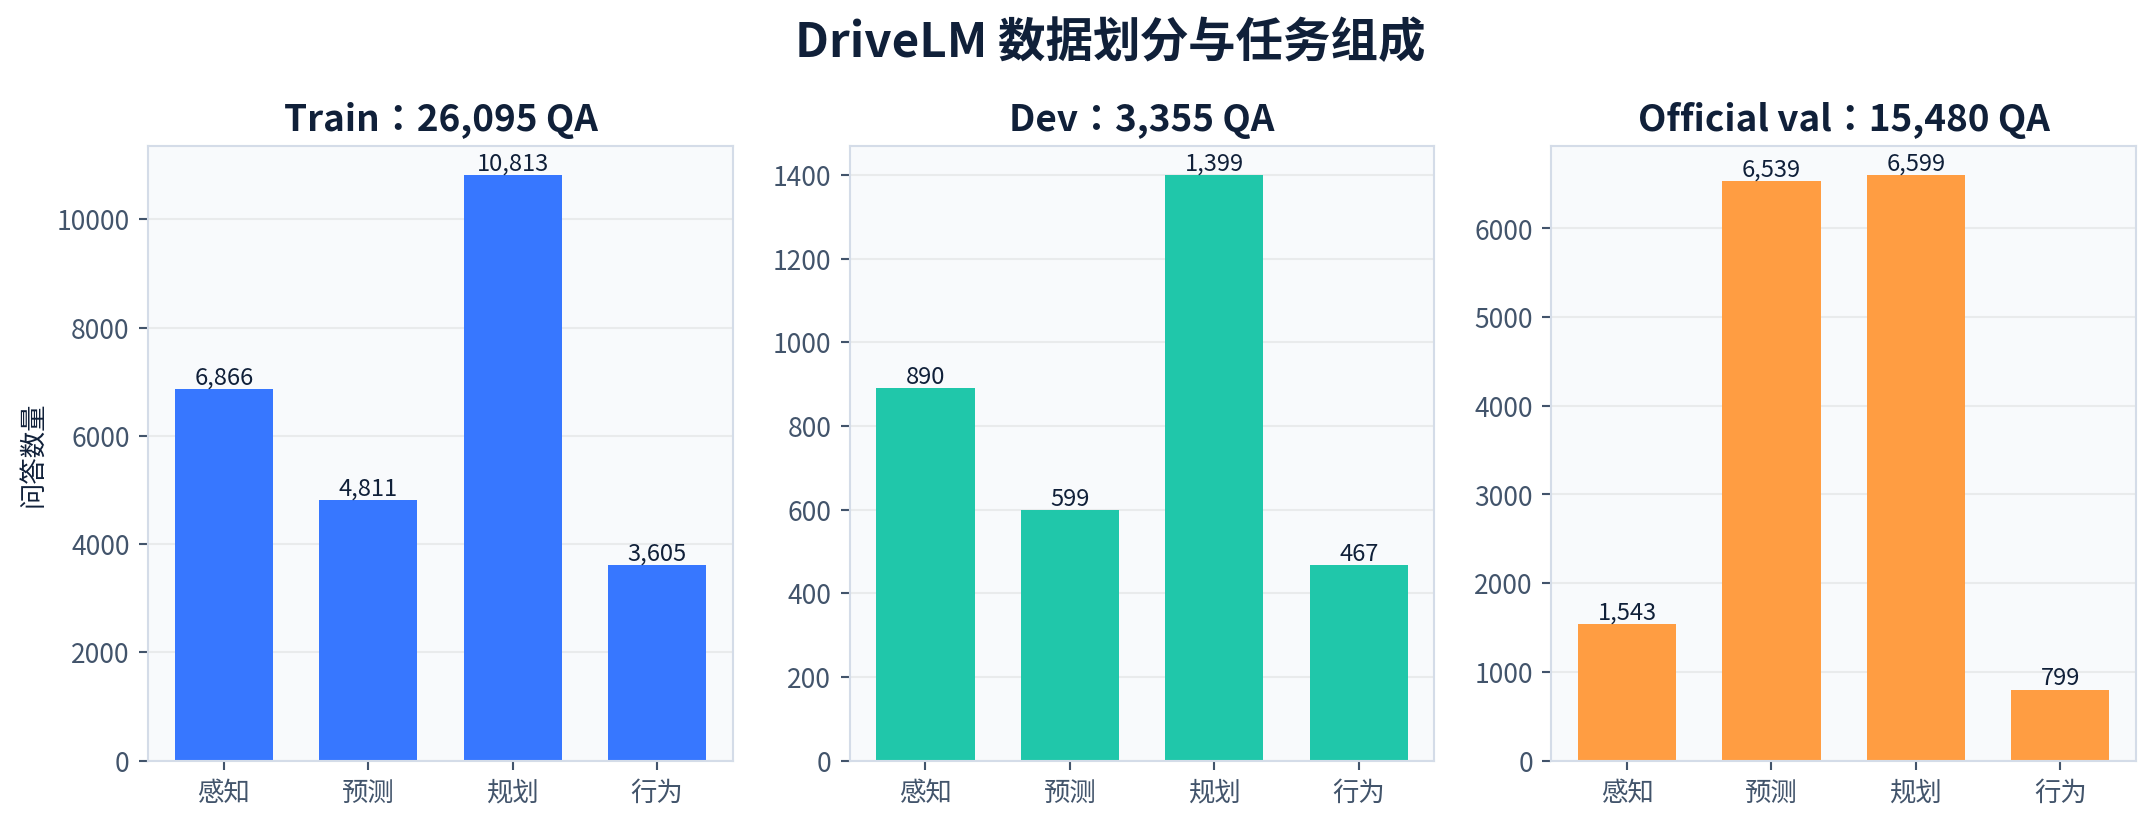
\includegraphics[width=0.94\textwidth]{dataset_task_distribution.png}
  \caption{训练、开发和官方 val 中四类任务的数量分布。}
\end{figure}

\subsection{JSONL 与监督边界}
每条独立 QA 样本包含 scene ID、frame ID、QA index、任务类型、六图路径和 system/user/assistant 消息。CE-SFT 只监督 assistant token，图像、system 和 user token 的 label 为 \(-100\)：
\[
\mathcal L_{\mathrm{CE}}
=-\sum_{t\in\mathrm{assistant}}
\log p_\theta(y_t\mid I_{1:6},q,y_{<t}).
\]
Graph-SFT 将同一帧的全部 QA 打包为多轮 trajectory；六张图只在首节点输入，后续节点读取上游 assistant 消息作为显式工作记忆。

\section{统一评测协议}
\subsection{为什么不能只看 Token-F1}
DriveLM 同时包含短分类答案、自由文本规划、对象坐标和图依赖。单一 lexical 指标无法反映：对象识别错误是否导致后续问题被 gating、同义规划是否语义正确、坐标是否匹配，以及模型是否只在较容易的有效子集上得分。因此主线同时报告离线 lexical 指标、结构指标、语义裁判和完整 Final。

\subsection{本地 DriveLM-DS}
本地 evaluator 沿用公开 challenge 的指标结构：
\[
S_{\mathrm{Final}}
=0.4S_{\mathrm{semantic}}
+0.2S_{\mathrm{language}}
+0.2S_{\mathrm{match}}
+0.2S_{\mathrm{accuracy}}.
\]
其中 semantic 使用 DeepSeek-V4-Flash、temperature 0，作为官方 ChatGPT Score 的本地代理；Language 由 BLEU-1--4、ROUGE-L 和 CIDEr 合成；Match 衡量重要对象与坐标结构；Accuracy 处理分类式问题。所有可比较候选要求 3,355/3,355 coverage 和 Judge completion 100\%。

\subsection{Graph gating 与 same-ID 公平审计}
每帧首个 important-object 回答决定哪些下游 QA 满足坐标 gating。两个模型可能拥有不同的 eligible 集合，直接比较 Full Final 会把“模型能力变化”和“题目集合变化”混在一起。项目因此固定执行：
\[
\mathcal I_{\mathrm{pair}}
=\mathcal I_{\mathrm{baseline}}\cap\mathcal I_{\mathrm{candidate}}.
\]
双方只在 \(\mathcal I_{\mathrm{pair}}\) 上重新计算指标，并要求 Final 严格提高，Planning、MC 与 coordinate F1 不超过预注册回退阈值。

\subsection{Predicted-context rollout}
Teacher-forced dev NLL 只回答“给定正确上游答案时，模型能否预测当前答案”。真实 Agent 没有 gold context，因此最终 Graph 评测必须执行：
\[
\hat y_1=f(I,q_1),\quad
\hat y_t=f(I,q_{1:t},\hat y_{1:t-1}).
\]
即把模型自己的 Perception/Prediction 输出继续输入 Planning/Behavior。该协议显式测量上游错误传播与 exposure mismatch；dev NLL 仅用于低成本 checkpoint screening，不用于最终晋级。

\section{技术演进与理论依据}
\subsection{阶段 0：零样本基模}
Qwen2.5-VL-7B-Instruct 原生支持多图，但未经 DriveLM 模板、对象 ID、坐标和规划语言适配。零样本 Final 仅 0.257961，说明通用视觉语言能力不能直接替代垂域格式与决策知识。该结果为后续所有改进提供冻结起点。

\subsection{阶段 1：六相机纯 CE-LoRA SFT}
首个稳定 7B 主线采用单帧六图、assistant-token-only CE 和 LoRA。LoRA rank 8、\(\alpha=16\)、dropout 0.05，目标模块包括注意力投影与 MLP 投影；adapter 包含视觉和语言两部分参数。在当前 7B 配置中，可训练参数 23,794,688，占 8,315,961,344 总参数的约 0.286\%。

纯 CE 的理论作用是最大化垂域答案似然，不把 dev Final、judge 或手写 metric 权重混进初始表示学习。B10 将 Final 从 0.257961 提升到 0.594636，是整个项目最大的单阶段增益，也验证“先建立强 CE 基线，再进行偏好或 RL 优化”的路线。

同阶段的高视觉预算 B11 反而下降到 0.580881。更多视觉 token 增加了计算量，却没有自动改善对象召回，说明瓶颈不仅是分辨率，还包括监督对齐、任务干扰与坐标格式。

\subsection{阶段 2：CE 锚定的保守 DPO}
标准 DPO 使用 7,149 组候选偏好对，优化 chosen 相对 rejected 的优势：
\[
\mathcal L_{\mathrm{DPO}}
=-\log\sigma\!\left(
\beta\left[
\log\frac{\pi_\theta(y^+\mid x)}{\pi_{\mathrm{ref}}(y^+\mid x)}
-\log\frac{\pi_\theta(y^-\mid x)}{\pi_{\mathrm{ref}}(y^-\mid x)}
\right]\right).
\]
标准 DPO-100 虽提高部分 lexical 与 MC 指标，但 Planning/judge 回退，Final 为 0.594300。问题表现为偏好分布不均和更新过强，而非 adapter 容量不足。

保守 DPO 将四任务偏好均衡，使用较小 \(\beta=0.05\)，并加入 chosen-answer CE anchor：
\[
\mathcal L=\mathcal L_{\mathrm{DPO}}+\lambda\mathcal L_{\mathrm{CE}}(y^+),
\qquad \lambda=0.1.
\]
CE anchor 相当于对原语言建模能力施加软约束，降低 preference over-optimization。checkpoint-75 的 Final 达到 0.596356；1,807-ID same-ID Final 同样提高 0.001056，因此正式晋级。

\subsection{阶段 3：Mixture of LoRA 专家分解}
单个 adapter 同时优化四类任务时，短分类、长规划与坐标 grounding 的梯度可能方向冲突。MoL 使用一个共享 7B 基座和四个任务 LoRA：
\[
e=r(q)\in\{P,Pr,Pl,B\},\qquad
h'=h+\Delta W_e h.
\]
路由 \(r(q)\) 只读取已知任务类型，而不是候选答案或 dev 分数，因此可部署且无答案依赖。每个专家仍用普通 CE 训练；改进来自参数子空间解耦，而不是将最终评测指标写入 loss。

自适应 controller 每 100 step 评估 Token-F1，同时设置 Planning、MC、anchor F1 安全门槛；step 800/900 连续未超过 step 700 的最小增益，触发 patience=2 并回滚。MoL-700 将 Final 提升到 0.608245，same-ID Final 提升 0.013886，是 SFT 后最重要的结构改进。

\subsection{阶段 4：Planning trajectory GRPO 与 GSPO}
项目把冻结的 Perception/Prediction 结果组织为 Planning trajectory 上下文，对 Planning 专家进行组相对策略优化。确定性奖励为：
\[
R=0.40F_{1,\mathrm{token}}+0.20R_{L}
+0.25F_{1,\mathrm{action}}+0.05\mathrm{EM}
+0.05V_{\mathrm{ground}}+0.05V_{\mathrm{format}}.
\]
GRPO 与 GSPO 共享数据、候选数、seed、reward 和训练预算，只改变 policy loss 聚合。GSPO-90 在 Planning 子协议上取得最高 reward 61.2600，优于 MoL control 60.8118 和 GRPO-70 61.1674。

然而接回四任务系统后，GRPO/GSPO Final 分别为 0.606702/0.606640，均低于 MoL-700。理论原因是局部 reward 优化与 graph-eligible Final 不完全一致；一个策略可以改善全体 Planning trajectory，却在官方 gating 后的 Planning 子集上退化。该实验说明 RL 的 reward 必须与最终部署分布和系统级晋级门槛联合验证。

\subsection{阶段 5：四阶段 Graph trajectory SFT}
Graph-SFT 将同一帧的全部节点打包为一条因果对话，所有 assistant span 计算 CE。下游 token loss 通过共享 attention 更新模型参数，使模型学习跨任务上下文；但离散上游文本本身不可微，不能把 Planning 的 token loss直接“反传成正确的 Perception 答案”。

Graph-A 将坐标 grounding 与 Match 显著提高，candidate-dependent Full Final 达到 0.609998；但在严格 1,848-ID 交集上 Final 下降 0.003428，Planning 与 MC 也下降，因此未晋级。核心问题是 teacher forcing：训练时下游看到 gold 上游答案，部署时看到模型预测，形成 exposure mismatch。Graph+CE-anchor 混合版本也未修复这一问题。

\subsection{阶段 6：受 InternVL4Drive 启发的固定专家路由}
InternVL4Drive 的可迁移洞见不是必须更换为 25.5B InternVL，而是利用互补模型：Grounding 强的模型负责感知瓶颈，推理强的模型负责下游。项目冻结路由：
\begin{lstlisting}
if qa_index == 0:
    answer = Graph_A(frame_anchor)
else:
    answer = MoL_700(task_expert)
\end{lstlisting}
路由只使用输入侧节点位置，不读取答案、reference、置信度或 dev 分数。Graph-A 负责 467 条 frame anchor；MoL-700 负责 2,888 条下游 QA。该组合把“坐标召回”和“规划语言”分配给各自优势专家，避免在同一个 adapter 内折中。

完整 Final 从 0.608245 提高到 0.612293；common 1,848-ID Final 从 0.609563 提高到 0.610557，全部 paired gates 通过。网络禁用的 cache-only Judge 完成 791/791 命中，保证本轮没有新增外发 payload。

\subsection{阶段 7：空间提示与 bbox 辅助负实验}
为验证 InternVL 的其他思路，v0.44 保持六张独立图输入，测试：
\begin{enumerate}
  \item \textbf{显式相机拓扑：}在 system prompt 中声明前、后、左右视角及相机内坐标系；
  \item \textbf{image-only bbox auxiliary：}训练时只输入原始六图，目标只输出相机名和归一化 bbox；不输入真实框、中心点、类别、状态或描述。视觉 LoRA 确实接收梯度。
\end{enumerate}
显式拓扑模型的 EM 与部分坐标指标略升，但 Token-F1、MC 和 eligible 数下降；接入“anchor+MoL”后仍略低于 v0.43。bbox 辅助模型的 anchor F1 降到 12.77\%，eligible 降到 1,883，Planning Token-F1 降到 57.57\%。可能原因包括辅助检测目标与 DriveLM center-point/graph 目标不一致、有限 LoRA 容量下的梯度干扰，以及“所有重要对象框”对最终语言规划并非充分统计量。两者均作为负实验保存，不调用额外语义 Judge，也不替换主线。

\section{统一性能演进}
\begin{table}[H]
\centering
\caption{3,355-QA 本地完整系统性能。Final 均为同一 DriveLM-DS 代理结构；\(\dagger\) 表示最终晋级。}
\scriptsize
\begin{tabular}{p{2.5cm}rrrrrrp{1.55cm}}
\toprule
模型阶段 & EM & Token-F1 & ROUGE-L & MC & Judge/100 & Final & 结论\\
\midrule
7B zero-shot & 13.71 & 24.23 & 21.74 & 51.69 & 36.83 & 0.257961 & control\\
CE-LoRA B10 & 43.46 & 73.00 & 71.08 & 83.82 & 70.63 & 0.594636 & \(\dagger\)\\
Standard DPO-100 & 43.55 & 73.17 & 71.22 & 84.27 & 69.75 & 0.594300 & 未晋级\\
Conservative DPO-75 & 43.58 & 73.12 & 71.20 & 84.16 & 70.86 & 0.596356 & \(\dagger\)\\
Grounding DPO-50 & -- & -- & -- & -- & 69.73 & 0.592092 & 未晋级\\
MoL-700 & 43.99 & 74.53 & 72.41 & 84.49 & 72.48 & 0.608245 & \(\dagger\)\\
GRPO-70 full system & 43.55 & 74.00 & 71.90 & 84.49 & 72.09 & 0.606702 & 未晋级\\
GSPO-90 full system & 43.79 & 74.02 & 71.94 & 84.49 & 72.08 & 0.606640 & 未晋级\\
Graph-A CE-600 & 43.04 & 73.04 & 71.00 & 83.71 & 71.30 & 0.609998 & same-ID 拒绝\\
Graph+anchor-600 & 42.62 & 72.56 & 70.55 & 83.48 & 70.70 & 0.605430 & 未晋级\\
\rowcolor{LightGreen}
Graph anchor + MoL & 43.99 & 74.48 & 72.38 & 84.49 & 73.02 & \textbf{0.612293} & \textbf{当前基线}\\
\bottomrule
\end{tabular}
\end{table}

\subsection{累计增益}
\begin{itemize}
  \item zero-shot \(\rightarrow\) CE-SFT：Final 绝对提升 0.336675，相对提升约 130.52\%；
  \item CE-SFT \(\rightarrow\) conservative DPO：提升 0.001721；
  \item conservative DPO \(\rightarrow\) MoL：提升 0.011889；
  \item MoL \(\rightarrow\) fixed anchor ensemble：提升 0.004048；
  \item zero-shot \(\rightarrow\) 当前系统：Final 从 0.257961 提升到 0.612293，绝对提升 0.354332。
\end{itemize}

\subsection{当前基线完整指标}
\begin{table}[H]
\centering
\caption{v0.43 完整 3,355-QA 官方风格本地指标。}
\begin{tabular}{lr@{\qquad}lr}
\toprule
指标 & 数值 & 指标 & 数值\\
\midrule
Coverage & 3,355/3,355 & Graph eligible & 1,927\\
Accuracy & 0.813154 & Semantic Judge & 73.0197\\
BLEU-1 & 0.789634 & BLEU-2 & 0.724770\\
BLEU-3 & 0.665099 & BLEU-4 & 0.607520\\
ROUGE-L & 0.724571 & CIDEr & 0.198875\\
Match /100 & 30.7513 & Final & \textbf{0.612293}\\
\bottomrule
\end{tabular}
\end{table}

\section{晋级制度与实验可信度}
\subsection{冻结门槛}
每个阶段在查看语义 Final 前先完成 lexical/structural screening，冻结候选选择规则。完整晋级要求：
\begin{enumerate}
  \item 3,355/3,355 coverage，空答案与重复 ID 为 0；
  \item 语义 Judge complete 100\%；
  \item Full Final 严格提高；
  \item same-ID Final 严格提高；
  \item Planning、MC、coordinate F1 不越过预注册回退阈值；
  \item 训练数据不包含 dev/hidden-val 答案，路由不使用 reference 或候选得分。
\end{enumerate}
这套门槛解释了为什么 Graph-A 的 raw Final 0.609998 高于 MoL 0.608245，却没有直接晋级：它在共同 1,848-ID 上退化。相反，v0.43 在 full 与 paired 两种口径上均提高，因此可以成为新基线。

\subsection{外部 Judge 与缓存边界}
官方 ChatGPT evaluator 在本地不可用，项目使用 DeepSeek-V4-Flash 作为语义代理；其数值不能与官方 leaderboard 直接等同。Judge 请求以 model、base URL、prompt version、candidate、reference 和 kind 形成哈希缓存键。cache-only evaluator 以 SQLite read-only 模式工作，任一 miss 立即失败，防止未授权数据发送。

\section{从正负实验得到的理论结论}
\begin{enumerate}
  \item \textbf{垂域 SFT 是必要条件。}通用 VLM 不熟悉 DriveLM 对象 ID、坐标、回答模板和决策语言；纯 CE 已解决大部分 domain gap。
  \item \textbf{偏好优化需要保留语言锚。}标准 DPO 容易过优化偏好边界；任务均衡与 chosen CE anchor 能降低灾难性漂移。
  \item \textbf{任务分解比单一共享 adapter 更有效。}MoL 的主要收益来自减少四任务之间的梯度冲突，且 hard router 比答案依赖 gate 更容易审计。
  \item \textbf{局部 reward 提升不代表全系统提升。}GRPO/GSPO 改善 Planning trajectory，但 graph gating 后的部署分布不同；系统级 Final 必须作为最终门控。
  \item \textbf{Graph 结构既是能力来源也是评测陷阱。}联合 trajectory 能改善 grounding，但 teacher forcing 会掩盖上游错误传播；必须使用 predicted-context 与 same-ID。
  \item \textbf{专家组合可优于继续训练。}v0.43 没有新增模型参数，只通过固定节点级路由组合 Graph-A 与 MoL 的互补优势，取得当前最大后期增益。
  \item \textbf{更多视觉监督并不自动更好。}提高 token、显式相机拓扑和 bbox 辅助均未晋级；辅助目标只有在与最终 graph/center-point 目标和采样分布一致时才可能有效。
\end{enumerate}

\section{工程复现与产物}
\subsection{核心目录}
\begin{lstlisting}
reproduction/qwen_vl_v036/                 # 7B pure CE SFT
reproduction/qwen_vl_v037b/                # conservative DPO + CE anchor
reproduction/qwen_vl_v039_mol/             # four LoRA experts + controller
reproduction/qwen_vl_v040_trajectory_rl/   # GRPO / GSPO
reproduction/qwen_vl_v042_graph/           # Graph-SFT + rollout
reproduction/qwen_vl_v043_internvl_transfer/ # fixed expert routing
reproduction/qwen_vl_v044_spatial_bbox/    # topology/bbox negative ablation
reproduction/drivelm_ds_eval/               # official-style local evaluator
results/leaderboard/                        # complete machine-readable table
\end{lstlisting}

\subsection{关键复现命令}
\begin{lstlisting}[language=bash]
# Build scene-isolated six-camera data
python reproduction/qwen_vl/build_dataset.py \\
  --train-json /mnt/data/zzy/drivelm/data/QA_dataset_nus/v1_1_train_nus.json \\
  --val-json /mnt/data/zzy/drivelm/data/QA_dataset_nus/v1_1_val_nus_q_only.json \\
  --output-dir /mnt/data/zzy/drivelm/reproduction/qwen_vl \\
  --seed 42 --dev-ratio 0.1

# Build the promoted v0.43 fixed router output
python reproduction/qwen_vl_v043_internvl_transfer/build_fixed_ensemble.py \\
  --references-jsonl /mnt/data/zzy/drivelm/reproduction/qwen_vl_stage2_ablation_v1/qwen_v033_c00_dev.jsonl \\
  --baseline-json /mnt/data/zzy/drivelm/reproduction/qwen_vl_v039_mol/sweep/checkpoint-700/mol_dev_predictions.json \\
  --grounding-json /mnt/data/zzy/drivelm/reproduction/qwen_vl_v042_graph/rollout_checkpoint600/graph_dev_predictions.json \\
  --mode anchor --output-json ensemble_predictions.json \\
  --report-json build_report.json

# Network-disabled semantic evaluation from an existing cache
python reproduction/drivelm_ds_eval/evaluate_cache_only.py \\
  --references-jsonl qwen_v033_c00_dev.jsonl \\
  --predictions-json ensemble_predictions.json \\
  --output-json drivelm_ds.json --cache-file deepseek_judge.sqlite
\end{lstlisting}

\subsection{可视化展示}
项目生成连续驾驶视频：画面正常播放，在关键问题处冻结并弹出模型问答，再继续播放。视频用于展示 Agent 交互和答案格式，不替代 dev 定量指标；画面中的标注框均明确标识来源。

\begin{figure}[H]
  \centering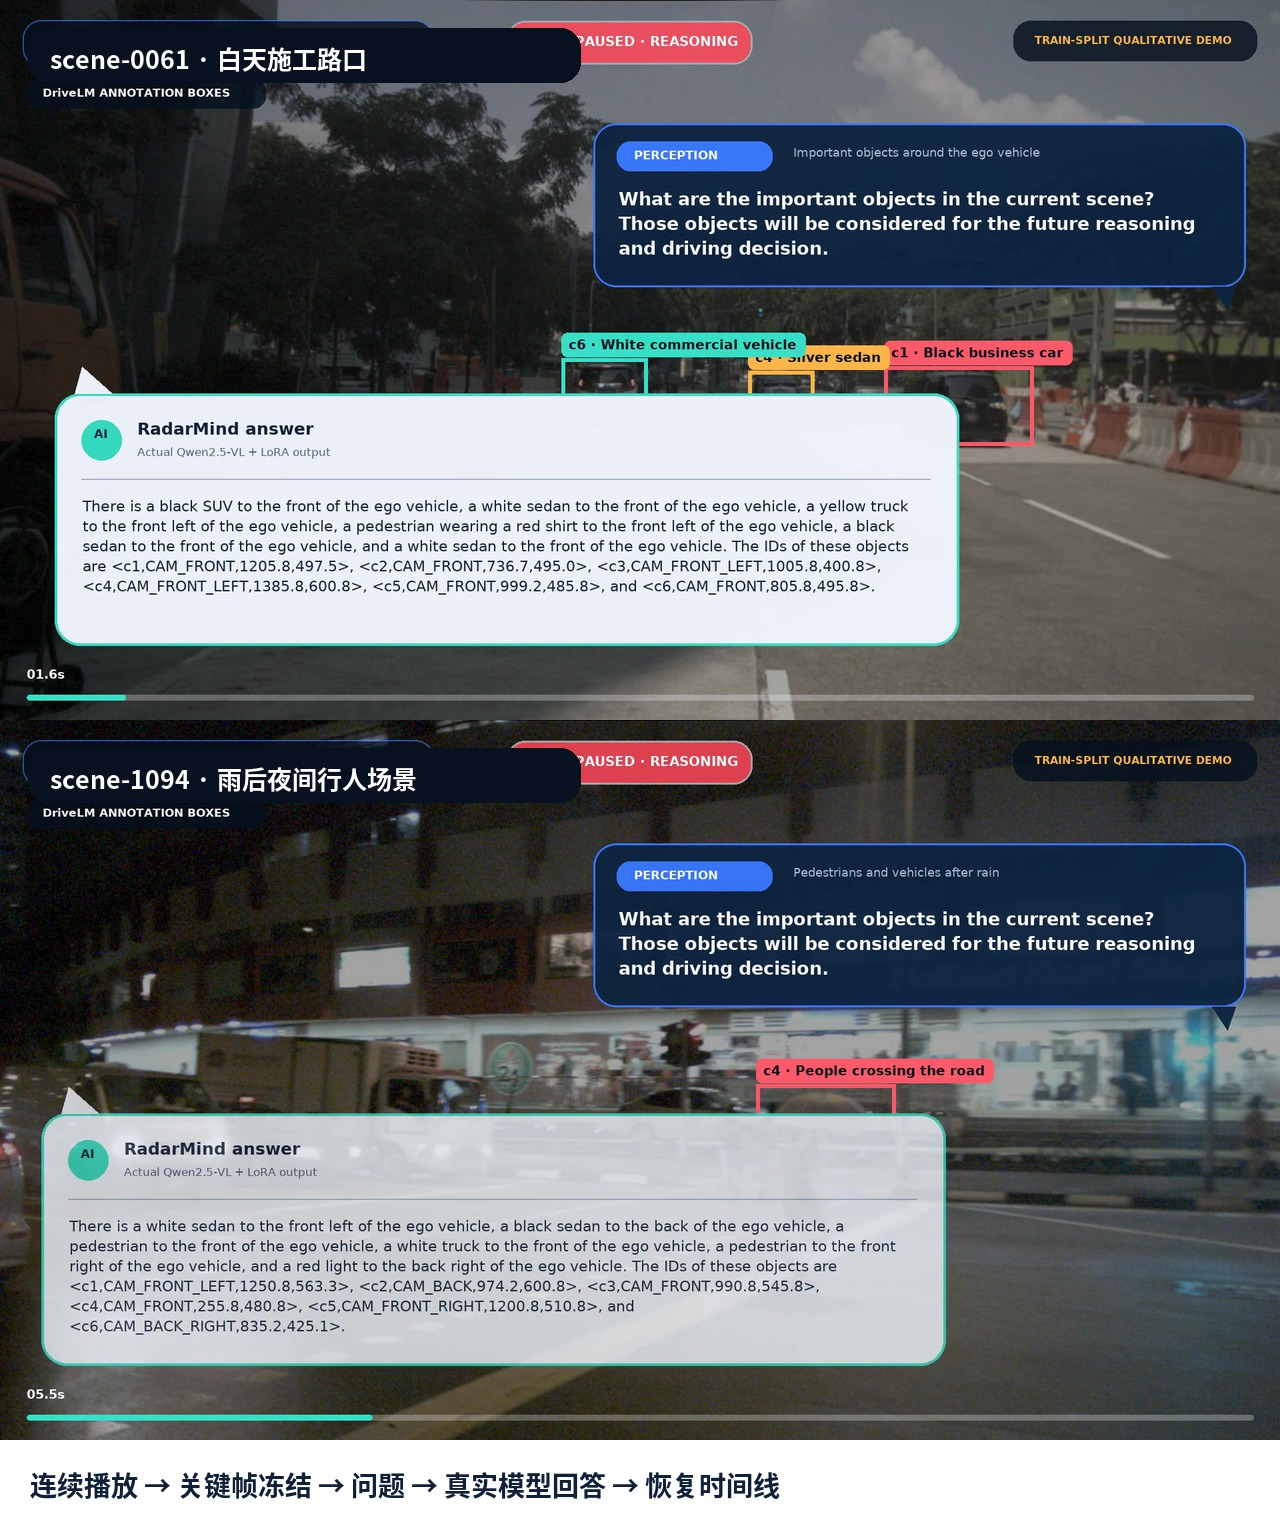
\includegraphics[width=0.92\textwidth]{qualitative_continuous_demos.jpg}
  \caption{两类昼夜场景的连续 DriveLM 问答展示。定性视频与定量 dev 评测严格分离。}
\end{figure}

\section{局限性与下一步}
\begin{itemize}
  \item 当前 Final 是 local dev + DeepSeek proxy，不是官方 hidden-server ChatGPT 分数；
  \item 主要实验为单 seed，尚未通过多随机种子给出置信区间；
  \item 单帧六相机难以可靠恢复真实速度、加速度和转向变化；
  \item Graph-SFT 仍有 teacher-forcing exposure mismatch；
  \item 当前主线是纯视觉 DriveLM，尚未把 radar token 纳入同一受控榜单；
  \item v0.43 依赖多个 LoRA adapter 的固定路由，服务端需要 adapter 缓存或高效切换。
\end{itemize}

推荐后续优先级：
\begin{enumerate}
  \item 在官方 val/test 服务器验证 v0.43，建立 local proxy 与官方分数的相关性；
  \item 对 Graph-SFT 使用 scheduled sampling 或 DAgger，把部分 gold context 替换为冻结模型预测；
  \item 直接优化 graph-eligible Planning 或使用双门控 reward，避免 RL 子协议与全系统错位；
  \item 对当前晋级链至少补充 3 个 seed，并报告 paired bootstrap 置信区间；
  \item 在不改变六相机基线的前提下增加 radar encoder，严格比较 camera-only、radar-only 与 fusion；
  \item 将最终 Planning 输出映射为结构化动作，并在 CARLA safety shield 下进行闭环验证。
\end{enumerate}

\section{结论}
RadarMind-DriveLM 已从“能运行的六相机 VQA 复现”演进为具有数据治理、分阶段训练、Graph rollout、系统级评测和公平晋级机制的自动驾驶 VLM Agent。最重要的工程结果不是某个单点算法，而是形成了可证伪的实验闭环：CE 建立垂域能力，保守 DPO 校准偏好，MoL 缓解任务冲突，RL 检查序列级优化，Graph-SFT暴露上游误差传播，最终用固定专家路由组合互补能力。

当前 v0.43 在本地完整协议上达到 \metric{0.612293}，相比零样本基模提升 0.354332；其 same-ID 增益证明提升并非来自 gating 子集变化。空间提示和 bbox 辅助的负结果也被完整保留，为后续 scheduled sampling、多模态雷达融合与 CARLA 闭环提供了明确边界。

\section*{参考资料}
\addcontentsline{toc}{section}{参考资料}
\begin{enumerate}
  \item Sima, C. et al. \textit{DriveLM: Driving with Graph Visual Question Answering}.\linebreak ECCV 2024; arXiv:2312.14150.
  \item Bai, S. et al. \textit{Qwen2.5-VL Technical Report}. arXiv:2502.13923, 2025.
  \item Caesar, H. et al. \textit{nuScenes: A Multimodal Dataset for Autonomous Driving}. CVPR 2020.
  \item Hu, E. J. et al. \textit{LoRA: Low-Rank Adaptation of Large Language Models}. ICLR 2022.
  \item Rafailov, R. et al. \textit{Direct Preference Optimization: Your Language Model is Secretly a Reward Model}. NeurIPS 2023.
  \item Shao, Z. et al. \textit{DeepSeekMath: Pushing the Limits of Mathematical Reasoning in Open Language Models}. arXiv:2402.03300, 2024（GRPO）.
  \item Li, J., Li, Z., Lu, T. \textit{Driving with InternVL}. CVPR 2024 Autonomous Grand Challenge technical report.
  \item OpenGVLab. \textit{InternVL: Scaling up Vision Foundation Models and Aligning for Generic Visual-Linguistic Tasks}. CVPR 2024.
\end{enumerate}

\appendix
\section{版本与决策索引}
\begin{longtable}{p{1.8cm}p{4.2cm}p{7.2cm}p{1.5cm}}
\toprule
版本 & 方法 & 主要证据 & 决策\\
\midrule
\endfirsthead
\toprule
版本 & 方法 & 主要证据 & 决策\\
\midrule
\endhead
v0.31 & 3B 初始复现 & 打通数据、LoRA、dev、官方 val 输出 & 历史起点\\
v0.36 & 7B CE-LoRA & Final 0.594636 & 晋级\\
v0.37A & Standard DPO & Final 0.594300 & 拒绝\\
v0.37B & Conservative DPO & Full 与 same-ID 均提高 & 晋级\\
v0.38A & Grounding DPO & Final 0.592092 & 拒绝\\
v0.39B & Four-expert MoL & Final 0.608245，controller 选 step 700 & 晋级\\
v0.40 & GRPO / GSPO & Planning 子协议提高，全系统下降 & 拒绝\\
v0.42A/B & Graph trajectory SFT & grounding 提高，same-ID 下降 & 拒绝\\
v0.43 & Graph anchor + MoL & Full 0.612293；paired +0.000993 & 晋级\\
v0.44 & topology / bbox auxiliary & 局部改善或整体退化 & 拒绝\\
\bottomrule
\end{longtable}

\section{v0.44 最新负实验明细}
\begin{table}[H]
\centering
\caption{不调用外部 Judge 的 3,355-QA predicted-context 离线结果。}
\begin{tabular}{lrrrrr}
\toprule
模型 & EM & Token-F1 & ROUGE-L & Planning F1 & MC\\
\midrule
Graph-A & 43.0402 & 73.0446 & 71.0026 & 58.3614 & 83.7079\\
显式相机拓扑 & 43.5768 & 73.0125 & 71.0570 & 58.3903 & 83.4831\\
相机拓扑+bbox & 43.0402 & 72.6065 & 70.6764 & 57.5701 & 83.3708\\
\bottomrule
\end{tabular}
\end{table}

显式拓扑作为 v0.43 anchor 替代时，EM 和 MC 与当前系统相同，但 Token-F1 从 74.4813\% 降到 74.4793\%，ROUGE-L 从 72.3789\% 降到 72.3573\%，eligible 从 1,927 降到 1,910；因此无需消耗额外 API Judge 即可在冻结 pre-gate 淘汰。

\section{报告再生成}
\begin{lstlisting}[language=bash]
cd /home/zhangzongyuan/Myproject/publish/radarmind-drivelm/reports/drivelm_reproduction_v1
xelatex -interaction=nonstopmode -halt-on-error drivelm_reproduction_technical_report.tex
xelatex -interaction=nonstopmode -halt-on-error drivelm_reproduction_technical_report.tex
\end{lstlisting}
\end{document}
